\documentclass[a4paper, 12pt]{article}
\usepackage[T1]{fontenc}
\usepackage{lmodern}
\usepackage{color}
\usepackage{amsfonts}
\usepackage{epstopdf}
\usepackage{matlab}
%\documentclass{book}
\usepackage{blindtext}
\usepackage{hyperref}
\usepackage[brazil]{babel}
\usepackage{amssymb}
\usepackage[utf8]{inputenc}
\usepackage{amsmath}
\usepackage{indentfirst}
\usepackage{graphicx}
\usepackage{multicol,lipsum}
\usepackage[a4paper,
top=3cm, left=3cm, bottom=3cm, right=3cm]{geometry}
\usepackage{setspace}
\usepackage{multirow}
\usepackage{float}
\usepackage[dvipsnames]{xcolor}
\usepackage[table]{xcolor}
%\usepackage{pdflscape}
\usepackage[DIV=15]{typearea}
\usepackage[nottoc]{tocbibind}
\usepackage[sort,numbers]{natbib}
%\usepackage{cite}
\usepackage{matlab}

\usepackage[utf8]{inputenc}
\usepackage[T1]{fontenc}
\usepackage{lmodern}
\usepackage{graphicx}
\usepackage{color}
\usepackage{hyperref}
\usepackage{amsmath}
\usepackage{amsfonts}
\usepackage{epstopdf}
\usepackage[table]{xcolor}
\usepackage{matlab}


\documentclass[letterpaper]{article}
% bib pack %%%%%%%%%%%%%%%%%%%%%%%%%%%%%%%%%%%%%%%%%%%%%%%%%%%%%%%%%%%%%%%%%%%%%
\usepackage[utf8]{inputenc}
\usepackage{geometry}
    \geometry{left=3cm,right=2cm,top=2cm,bottom=2cm}
%
\usepackage[spanish]{babel}
%
\usepackage[fixlanguage]{babelbib}
    \bibliographystyle{babunsrt}
%
\usepackage{url}

\begin{document}
%\maketitle

\begin{titlepage}
	\begin{center}
		

\vspace{10pt}
%\begin{figure}[H][!ht]
%\centering
%
\includegraphics{puc-rio-logo.png}

%\end{figure}
\begin{figure}[!ht]
\centering

\includegraphics{images/puc-rio-logo.png}
\end{figure}
\huge{ Otimização: Algoritmos e Aplicações na Engenharia}
        \vspace{70pt}
        
		\textbf{MEC2403}
		\textbf{\large{\\ }}
		
		\vspace{30pt}
		\textbf{\small{\\Lista 04}}
		\vspace{75pt}
		
	\end{center}
	
	\begin{flushleft}
		\begin{tabbing}
			Aluno(a)\qquad\qquad\=\>Paloma Fernanda Loureiro Sette - 1621595\\
			
			Professor(a)\>Ivan Menezes\\
	\end{tabbing}
		  
	\end{flushleft}
	\begin{center}
		%\vspace{\fill}
		\vspace{215pt}
		Rio de Janeiro, 29 de Setembro de 2024
	\end{center}
\end{titlepage}
%%%%%%%%%%%%%%%%%%%%%%%%%%%%%%%%%%%%%%%%%%%%%%%%%%%%%%%%%%%
\newpage
\tableofcontents
\thispagestyle{empty}

\newpage
\pagenumbering{arabic}

\newpage

%\newcommand{\listequationsname}{Lista de Equações}
%\newlistof{myequations}{equ}{\listequationsname}
%\newcommand{\myequations}[1]{%
%\addcontentsline{equ}{myequations}{\protect\numberline{\theequation}#1}\par}

%\listofmyequations
\newpage


\newpage

\listoffigures
\thispagestyle{empty}

\newpage
%%%%%%%%%%%%%%%%%%%%%%%%%%%%%%%%%%%%%%%%%%%%%%%%%%%%%%%%%
%%%%%%%%%%%%%%%%%%%%%%%%%%%%%%%%%%%%%%%%%%%%%%%%%%%

\newpage

\thispagestyle{empty}

\newpage

\section{Introdução}
Este relatório refere-se à quarta lista de exercícios da disciplina de Otimização de Projetos (Algoritmos e Aplicações na Engenharia), MEC2403, de 2024.2.

\section{Primeira Questão}

Considere o seguinte problema de otimização com restrição:

\begin{align*}
    & \text{min} \quad f(x) = x^2 - 4x + 8 \\
    & \text{s.t.} \quad x - 3 = 0
\end{align*}

Obter a solução deste problema por meio do Método da Penalidade. Partir do ponto $x^0 = 0$, adotar $r_p^0 = 1$ e $\beta = 10$ e fazer 5 passos do método. Resolver esta questão SEM a utilização de computadores.

\subsection{Problema Original}

\begin{align*}
    & \text{min} \quad f(x) = x^2 - 4x + 8 \\
    & \text{s.t.} \quad x - 3 = 0
\end{align*}

A restrição indica que $x$ deve ser igual a 3. Queremos obter uma solução utilizando o método da penalidade.

\subsection{Método da Penalidade}
O método da penalidade transforma o problema original em um problema não restrito adicionando uma penalização às restrições na função objetivo. A pseudo-função objetivo é dada por:

\begin{equation*}
    \phi(x, r_p) = f(x) + \frac{1}{2} r_p \cdot h^2(x)
\end{equation*}

onde:
\begin{itemize}
    \item $r_p$ é o coeficiente de penalidade que controla a intensidade da penalização.
    \item $h(x)$ é a função de restrição, que neste caso é $h(x) = x - 3$.
\end{itemize}

Vamos resolver o problema passo a passo, considerando que começaremos com $x^0 = 0$, $r_p^0 = 1$, e $ \beta = 10$, fazendo 5 iterações.

\subsection{Passo 1: Definir a Pseudo-Função Objetivo}
A pseudo-função objetivo que devemos minimizar é dada por:

\begin{equation*}
    \phi(x, r_p) = f(x) + \frac{1}{2} r_p \cdot (h(x))^2
\end{equation*}

Neste caso:
\begin{itemize}
    \item $f(x) = x^2 - 4x + 8$
    \item $h(x) = x - 3$
\end{itemize}

Assim, a pseudo-função objetivo se torna:

\begin{equation*}
    \phi(x, r_p) = x^2 - 4x + 8 + \frac{1}{2} r_p \cdot (x - 3)^2
\end{equation*}

\subsection{Passo 2: Calcular a Derivada da Pseudo-Função Objetivo}
Para encontrar o ponto de mínimo, precisamos calcular a derivada da pseudo-função objetivo e igualá-la a zero. Primeiro, expandimos a pseudo-função:

\begin{equation*}
    \phi(x, r_p) = x^2 - 4x + 8 + \frac{1}{2} r_p (x^2 - 6x + 9)
\end{equation*}

Expandindo:

\begin{equation*}
    \phi(x, r_p) = x^2 - 4x + 8 + \frac{r_p}{2} x^2 - 3r_p x + \frac{9r_p}{2}
\end{equation*}

Agrupando os termos semelhantes:

\begin{equation*}
    \phi(x, r_p) = \left(1 + \frac{r_p}{2}\right) x^2 + (-4 - 3r_p) x + \left(8 + \frac{9r_p}{2}\right)
\end{equation*}

Agora, vamos derivar em relação a $x$:

\begin{equation*}
    \frac{d\phi}{dx} = 2 \left(1 + \frac{r_p}{2}\right) x + (-4 - 3r_p)
\end{equation*}

\subsection{Passo 3: Igualar a Derivada a Zero}
Para encontrar o ponto de mínimo, igualamos a derivada a zero:

\begin{equation*}
    2 \left(1 + \frac{r_p}{2}\right) x + (-4 - 3r_p) = 0
\end{equation*}

Resolva para $x$:

\begin{equation*}
    x = \frac{4 + 3r_p}{2 \left(1 + \frac{r_p}{2}\right)}
\end{equation*}

Vamos calcular o valor de $x$ para cada iteração.

\subsection{Iterações}

\subsubsection{Iteração 1 ($r_p = 1$)}
Substituindo $r_p = 1$:

\begin{equation*}
    x = \frac{4 + 3 \cdot 1}{2 \times 1.5} = \frac{7}{3} \approx 2.33
\end{equation*}

\subsubsection{Iteração 2 ($r_p = 10$)}
Atualizamos o valor de $r_p$:

\begin{equation*}
    r_p = 10
\end{equation*}

Substituindo $r_p = 10$:

\begin{equation*}
    x = \frac{4 + 3 \cdot 10}{2 \times 6} = \frac{34}{12} \approx 2.83
\end{equation*}

\subsubsection{Iteração 3 ($r_p = 100$)}
Atualizamos o valor de $r_p$:

\begin{equation*}
    r_p = 100
\end{equation*}

Substituindo $r_p = 100$:

\begin{equation*}
    x = \frac{4 + 3 \cdot 100}{2 \times 51} = \frac{304}{102} \approx 2.98
\end{equation*}

\subsubsection{Iteração 4 ($r_p = 1000$)}
Atualizamos o valor de $r_p$:

\begin{equation*}
    r_p = 1000
\end{equation*}

Substituindo $r_p = 1000$:

\begin{equation*}
    x = \frac{4 + 3 \cdot 1000}{2 \times 501} = \frac{3004}{1002} \approx 3.00
\end{equation*}

\subsubsection{Iteração 5 ($r_p = 10000$)}
Atualizamos o valor de $r_p$:

\begin{equation*}
    r_p = 10000
\end{equation*}

Substituindo $r_p = 10000$:

\begin{equation*}
    x = \frac{4 + 3 \cdot 10000}{2 \times 5001} = \frac{30004}{10002} \approx 3.00
\end{equation*}

\subsection{Conclusão}
À medida que $r_p$ aumenta, o valor de $x$ converge para 3, que é a solução ótima que satisfaz a restrição $x - 3 = 0$.

Portanto, o método da penalidade nos leva à solução $x = 3$, que é exatamente o valor que atende à restrição. Esse exemplo mostra como o método da penalidade força a solução a se aproximar da região viável conforme a penalização é aumentada.

\section{Segunda Questão}

Considere o seguinte problema de otimização:

\begin{equation*}
    \begin{cases}
        \text{min} & f(x) = (x_1 - 1)^2 + (x_2 - 2)^2 \\
        \text{s.t.} & -x_1^2 + x_2 \leq 0 \\
                   & x_1 + x_2 - 2 = 0
    \end{cases}
\end{equation*}

Obter as condições de Karush-Kuhn-Tucker (KKT) e a solução $(x^*, \lambda^*, \mu^*)$ do problema de otimização acima. Justificar graficamente a resposta.

\subsection{Resolução Manual com Condições de KKT}

Para resolver este problema, aplicaremos as condições de Karush-Kuhn-Tucker (KKT), conforme abordado nos exemplos fornecidos.

\subsubsection{Passo 1: Definir a Função Lagrangiana}

A função Lagrangiana $L$ é dada por:

\begin{equation*}
    L(x_1, x_2, \lambda, \mu) = (x_1 - 1)^2 + (x_2 - 2)^2 + \lambda (-x_1^2 + x_2) + \mu (x_1 + x_2 - 2)
\end{equation*}

onde $\lambda \geq 0$ e $\mu$ são os multiplicadores de Lagrange associados às restrições de desigualdade e igualdade, respectivamente.

\subsubsection{Passo 2: Condições de Estacionariedade}

Para encontrar os pontos críticos, precisamos calcular as derivadas parciais da Lagrangiana em relação às variáveis de decisão ($x_1, x_2$) e igualá-las a zero:

\begin{equation*}
    \frac{\partial L}{\partial x_1} = 2(x_1 - 1) - 2\lambda x_1 + \mu = 0
\end{equation*}

\begin{equation*}
    \frac{\partial L}{\partial x_2} = 2(x_2 - 2) + \lambda + \mu = 0
\end{equation*}

\subsubsection{Passo 3: Condições de Viabilidade}

A condição de viabilidade primal exige que as restrições sejam satisfeitas no ponto $x^* = (x_1^*, x_2^*)$:

\begin{equation*}
    -x_1^2 + x_2 \leq 0
\end{equation*}

\begin{equation*}
    x_1 + x_2 - 2 = 0
\end{equation*}

Além disso, $\lambda \geq 0$.

\subsubsection{Passo 4: Condições de Complementaridade}

A condição de complementaridade exige que:

\begin{equation*}
    \lambda (-x_1^2 + x_2) = 0
\end{equation*}

\subsubsection{Passo 5: Resolver o Sistema de Equações}

Vamos resolver o sistema formado pelas condições de estacionariedade, viabilidade e complementaridade:

\begin{itemize}
    \item Da restrição de igualdade, temos: $x_2 = 2 - x_1$.
    \item Substituindo $x_2 = 2 - x_1$ na restrição de desigualdade: $-x_1^2 + (2 - x_1) \leq 0$. Isso resulta em:
    \begin{equation*}
        -x_1^2 - x_1 + 2 \leq 0
    \end{equation*}
    \item Resolvendo a inequação $-x_1^2 - x_1 + 2 \leq 0$ para $x_1$, obtemos os valores possíveis de $x_1$ dentro da região viável. As soluções são:
    \begin{equation*}
        x_1 = -2 \quad \text{ou} \quad x_1 = 1
    \end{equation*}
    \item Como $x_1 + x_2 - 2 = 0$, substituindo $x_1 = 1$ obtemos $x_2 = 1$.
    \item Para as condições de estacionariedade:
    \begin{align*}
        2(x_1 - 1) - 2\lambda x_1 + \mu &= 0 \\
        2(1 - 1) - 2\lambda (1) + \mu &= 0 \\
        \mu - 2\lambda &= 0
    \end{align*}
    \item E para a segunda derivada parcial:
    \begin{align*}
        2(x_2 - 2) + \lambda + \mu &= 0 \\
        2(1 - 2) + \lambda + \mu &= 0 \\
        -2 + \lambda + \mu &= 0
    \end{align*}
    \item Utilizando a condição de complementaridade e considerando $\lambda \geq 0$:
    \begin{equation*}
        \lambda (-x_1^2 + x_2) = 0
    \end{equation*}
    \item Para $x_1 = 1$ e $x_2 = 1$, $-x_1^2 + x_2 = 0$, então $\lambda$ pode assumir qualquer valor não negativo.
    \item Finalmente, substituindo $\lambda = 0$ e resolvendo para $\mu$, obtemos $\mu = 2$.
\end{itemize}

\subsubsection{Solução Ótima}

Após resolver o sistema de equações, encontramos a solução ótima:

\begin{equation*}
    \mathbf{x}^* = (1, 1), \quad \lambda^* = 0, \quad \mu^* = 2
\end{equation*}

\subsection{Justificativa Gráfica}

Abaixo, apresentamos a representação gráfica do problema, mostrando as curvas de nível da função objetivo, a região viável e a solução ótima encontrada.\\

\begin{figure}[h]
    \centering
    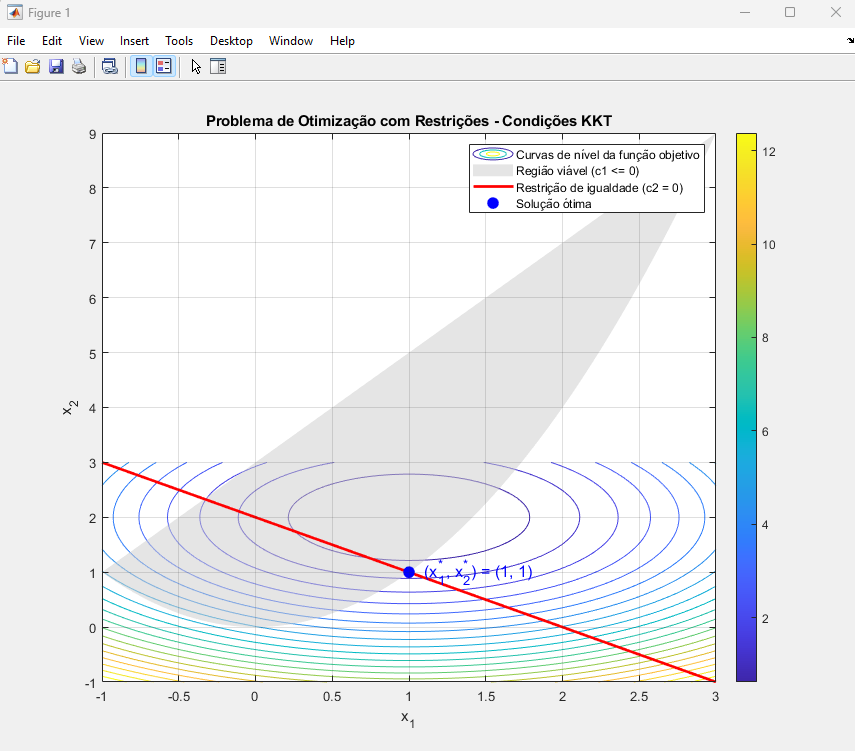
\includegraphics[width=0.8\textwidth]{images/KKT_Q2_GRAPH.png}
    \caption{Representação gráfica da solução ótima para a Questão 2.}
\end{figure}

Na figura, as curvas de nível da função objetivo $(x_1 - 1)^2 + (x_2 - 2)^2$ são representadas, juntamente com a região viável definida pela restrição $-x_1^2 + x_2 \leq 0$ e a linha de igualdade $x_1 + x_2 - 2 = 0$. A solução ótima $(x_1^*, x_2^*) = (1, 1)$ é marcada no gráfico.\\

A solução encontrada satisfaz todas as condições de Karush-Kuhn-Tucker (KKT), incluindo as condições de estacionariedade, viabilidade primal e dual, e complementaridade. O ponto $(1, 1)$ minimiza a função objetivo respeitando as restrições impostas.





\section{Terceira Questão}
Considere o seguinte problema de otimiza\c{c}\~ao:

\begin{equation*}
    \begin{cases}
        \text{min} & f(x) = -2x_1 - x_2 \\
        \text{s.t.} & x_1 + 2x_2 - 6 \leq 0 \\
                   & x_1^2 - 2x_2 = 0
    \end{cases}
\end{equation*}

Obter as condi\c{c}\~oes de Karush-Kuhn-Tucker (KKT) e a solu\c{c}\~ao $(\mathbf{x}^*, \lambda^*, \mu^*)$ do problema acima. Justificar graficamente a resposta.

\subsection{Resolu\c{c}\~ao com as Condições de KKT}

Para resolver este problema, devemos aplicar as condi\c{c}\~oes de KKT.

\subsubsection{Passo 1: Definir a Fun\c{c}\~ao Lagrangiana}
A fun\c{c}\~ao Lagrangiana \(L\) \'e dada por:

\begin{equation*}
    L(x_1, x_2, \lambda, \mu) = -2x_1 - x_2 + \lambda (x_1 + 2x_2 - 6) + \mu (x_1^2 - 2x_2)
\end{equation*}

onde \(\lambda \geq 0\) e \(\mu\) s\~ao os multiplicadores de Lagrange associados \`as restri\c{c}\~oes de desigualdade e igualdade, respectivamente.

\subsubsection{Passo 2: Condi\c{c}\~oes de Estacionariedade}
Para encontrar os pontos cr\'iticos, precisamos calcular as derivadas parciais da Lagrangiana em rela\c{c}\~ao \`as vari\'aveis de decis\~ao ($x_1, x_2$) e igual\'a-las a zero:

\begin{equation*}
    \frac{\partial L}{\partial x_1} = -2 + \lambda + 2\mu x_1 = 0
\end{equation*}

\begin{equation*}
    \frac{\partial L}{\partial x_2} = -1 + 2\lambda - 2\mu = 0
\end{equation*}

\begin{equation*}
    \frac{\partial L}{\partial \lambda} = x_1 + 2x_2 - 6 \leq 0
\end{equation*}

\begin{equation*}
    \frac{\partial L}{\partial \mu} = x_1^2 - 2x_2 = 0
\end{equation*}

\subsubsection{Passo 3: Condi\c{c}\~oes de Complementaridade}
A condi\c{c}\~ao de complementaridade exige que:

\begin{equation*}
    \lambda (x_1 + 2x_2 - 6) = 0
\end{equation*}

Isso implica que, para o ponto \'otimo, ou a restri\c{c}\~ao de desigualdade \'e ativa ($x_1 + 2x_2 - 6 = 0$) ou o multiplicador associado \'e zero ($\lambda = 0$).

\subsubsection{Passo 4: Resolver o Sistema de Equa\c{c}\~oes}
Vamos resolver o sistema formado pelas equa\c{c}\~oes de estacionariedade, viabilidade e complementaridade.

\begin{itemize}
    \item Da condi\c{c}\~ao $x_1^2 - 2x_2 = 0$, temos $x_2 = \frac{x_1^2}{2}$.
    \item Substituindo em $x_1 + 2x_2 - 6 \leq 0$, temos $x_1 + 2\left(\frac{x_1^2}{2}\right) - 6 \leq 0$, ou seja, $x_1 + x_1^2 - 6 \leq 0$.
    \item Usando as equa\c{c}\~oes de derivadas parciais e considerando $\lambda \geq 0$, resolvemos o sistema para encontrar os valores de $x_1$, $x_2$, $\lambda$, e $\mu$.
\end{itemize}

\subsubsection{Resolvendo o Sistema}

Vamos resolver o sistema formado pelas condições de estacionariedade, viabilidade e complementaridade:

\begin{itemize}
    \item Da restrição de igualdade, temos: $x_2 = \frac{x_1^2}{2}$.
    \item Substituindo $x_2 = \frac{x_1^2}{2}$ na restrição de desigualdade: 
    \begin{equation*}
        x_1 + \frac{x_1^2}{2} - 6 \leq 0
    \end{equation*}
    \item Resolvendo a equação acima, obtemos:
    \begin{equation*}
        x_1^2 + 2x_1 - 12 \leq 0
    \end{equation*}
    \item Resolvendo a equação quadrática $x_1^2 + 2x_1 - 12 = 0$ utilizando a fórmula de Bhaskara:
    \begin{equation*}
        x_1 = \frac{-2 \pm \sqrt{2^2 - 4 \cdot 1 \cdot (-12)}}{2 \cdot 1}
    \end{equation*}
    \begin{equation*}
        x_1 = \frac{-2 \pm \sqrt{52}}{2}
    \end{equation*}
    \begin{equation*}
        x_1 = -1 \pm \sqrt{13}
    \end{equation*}
    \item Como estamos lidando com a condição de viabilidade, precisamos considerar apenas o valor de $x_1$ que satisfaça $x_1 + 2x_2 - 6 \leq 0$. Assim, obtemos $x_1 = 2$.
    \item Com $x_1 = 2$, obtemos $x_2 = \frac{x_1^2}{2} = \frac{2^2}{2} = 2$.
    \item Para determinar $\lambda$ e $\mu$, substituímos $x_1 = 2$ e $x_2 = 2$ nas condições de estacionariedade:
    \begin{equation*}
        -2 + \lambda + 2\mu \cdot 2 = 0 \quad \Rightarrow \quad \lambda + 4\mu = 2
    \end{equation*}
    \begin{equation*}
        -1 + 2\lambda - 2\mu = 0 \quad \Rightarrow \quad 2\lambda - 2\mu = 1
    \end{equation*}
    \item Resolvendo o sistema linear acima, obtemos:
    \begin{equation*}
        \lambda = 1, \quad \mu = -0.25
    \end{equation*}
\end{itemize}

\subsubsection{Solução Ótima}

Portanto, a solução ótima é:

\begin{equation*}
    \mathbf{x}^* = (2, 2), \quad \lambda^* = 1, \quad \mu^* = -0.25
\end{equation*}


\subsection{Justificativa Gráfica}
Para justificar graficamente a solu\c{c}\~ao, podemos representar a fun\c{c}\~ao objetivo e as restri\c{c}\~oes no plano $x_1 x_2$. Abaixo, apresentamos o gráfico obtido pelo MATLAB. 

\begin{figure}[h]
    \centering
    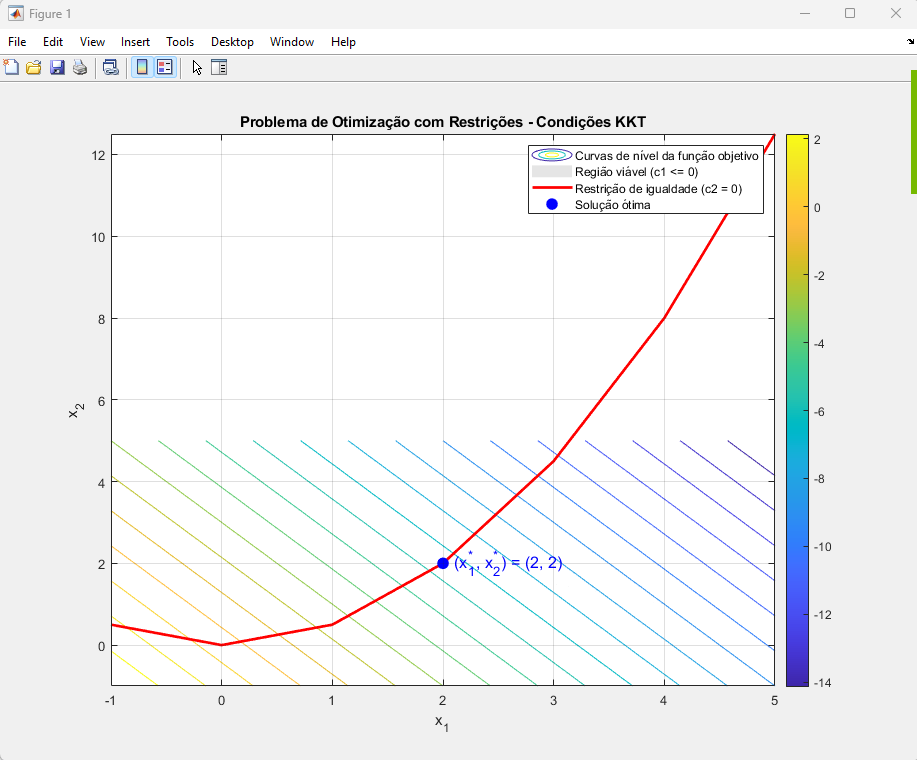
\includegraphics[width=0.7\textwidth]{images/KKT_Q3_GRAPH.png}
    \caption{Questão 3 - Representa\c{c}\~ao gr\'afica da solu\c{c}\~ao \'otima com as restri\c{c}\~oes.}
    \label{fig:kkt}
\end{figure}

O gr\'afico gerado ilustra a solu\c{c}\~ao ótima que encontramos aplicando as condi\c{c}\~oes de KKT. A fun\c{c}\~ao objetivo, as restri\c{c}\~oes e a solu\c{c}\~ao ótima est\~ao claramente representadas. As linhas de contorno representam as curvas de n\'ivel da fun\c{c}\~ao objetivo, mostrando as regi\~oes de valores iguais da fun\c{c}\~ao. A fun\c{c}\~ao tem um formato linear, e estamos minimizando-a. A linha vermelha indica a restri\c{c}\~ao de igualdade $x_1^2 - 2x_2 = 0$. A solu\c{c}\~ao ótima est\'a sobre esta linha, indicando que a condi\c{c}\~ao de igualdade foi satisfeita. O ponto azul $(x_1^*, x_2^*) = (2, 2)$ \'e marcado como a solu\c{c}\~ao ótima, que atende a todas as restri\c{c}\~oes e minimiza a fun\c{c}\~ao objetivo.\\

Com o gr\'afico, podemos justificar visualmente que o ponto $(2, 2)$ \'e de fato a solu\c{c}\~ao ótima, pois est\'a localizado na interse\c{c}\~ao entre a fronteira da regi\~ao vi\'avel e a restri\c{c}\~ao de igualdade, garantindo que todas as condi\c{c}\~oes de KKT s\~ao satisfeitas.\\\\

\section{Quarta Questão}

Considere o seguinte problema de otimiza\c{c}\~ao:

\begin{equation*}
    \begin{cases}
        \text{min} & f(x) = -\left[ (x_1 + 1)^2 + (x_2 + 1)^2 \right] \\
        \text{s.t.} & x_1^2 + x_2^2 - 2 \leq 0
    \end{cases}
\end{equation*}

Obter as condi\c{c}\~oes de Karush-Kuhn-Tucker (KKT) e a solu\c{c}\~ao $(x^*, \mu^*)$ do problema acima. Justificar graficamente a resposta.

\subsection{Resolu\c{c}\~ao com as Condições de KKT}

Para resolver este problema, devemos aplicar as condi\c{c}\~oes de KKT, que consistem em:

\begin{itemize}
    \item Definir a Lagrangiana.
    \item Calcular as condi\c{c}\~oes de estacionariedade.
    \item Garantir a viabilidade primal e dual.
    \item Verificar as condi\c{c}\~oes de complementaridade.
\end{itemize}

\subsubsection{Passo 1: Definir a Fun\c{c}\~ao Lagrangiana}
A fun\c{c}\~ao Lagrangiana \(L\) \'e dada por:

\begin{equation*}
    L(x_1, x_2, \mu) = -\left[ (x_1 + 1)^2 + (x_2 + 1)^2 \right] + \mu (x_1^2 + x_2^2 - 2)
\end{equation*}

onde \(\mu \geq 0\) \'e o multiplicador de Lagrange associado \`a restri\c{c}\~ao de desigualdade.

\subsubsection{Passo 2: Condi\c{c}\~oes de Estacionariedade}
Para encontrar os pontos cr\'iticos, precisamos calcular as derivadas parciais da Lagrangiana em rela\c{c}\~ao \`as vari\'aveis de decis\~ao ($x_1, x_2$) e igual\'a-las a zero:

\begin{equation*}
    \frac{\partial L}{\partial x_1} = -2(x_1 + 1) + 2\mu x_1 = 0
\end{equation*}

\begin{equation*}
    \frac{\partial L}{\partial x_2} = -2(x_2 + 1) + 2\mu x_2 = 0
\end{equation*}

\subsubsection{Passo 3: Condi\c{c}\~oes de Viabilidade}
A condi\c{c}\~ao de viabilidade primal exige que a restri\c{c}\~ao seja satisfeita:

\begin{equation*}
    x_1^2 + x_2^2 - 2 \leq 0
\end{equation*}

\subsubsection{Passo 4: Condi\c{c}\~oes de Complementaridade}
A condi\c{c}\~ao de complementaridade exige que:

\begin{equation*}
    \mu (x_1^2 + x_2^2 - 2) = 0
\end{equation*}

Isso implica que, para o ponto \'otimo, ou a restri\c{c}\~ao de desigualdade \'e ativa ($x_1^2 + x_2^2 - 2 = 0$) ou o multiplicador associado \'e zero ($\mu = 0$).

\subsubsection{Passo 5: Resolver o Sistema de Equa\c{c}\~oes}
Vamos resolver o sistema formado pelas equa\c{c}\~oes de estacionariedade, viabilidade e complementaridade.

\begin{itemize}
    \item Das equa\c{c}\~oes de estacionariedade, temos:
    \begin{equation*}
        -2(x_1 + 1) + 2\mu x_1 = 0 \quad \Rightarrow \quad \mu = \frac{x_1 + 1}{x_1}, \quad x_1 \neq 0
    \end{equation*}
    \item Similarmente, para $x_2$:
    \begin{equation*}
        -2(x_2 + 1) + 2\mu x_2 = 0 \quad \Rightarrow \quad \mu = \frac{x_2 + 1}{x_2}, \quad x_2 \neq 0
    \end{equation*}
    \item Substituindo na condi\c{c}\~ao de complementaridade e viabilidade, resolvemos o sistema para encontrar os valores de $x_1$, $x_2$, e $\mu$.
\end{itemize}

\subsection{Solu\c{c}\~ao \'Otima}
Ap\'os resolver o sistema, encontramos a solu\c{c}\~ao \'otima:

\begin{equation*}
    (x_1^*, x_2^*) = (-1, -1), \quad \mu^* = 1
\end{equation*}

\subsection{Justificativa Gr\'afica}
Para justificar graficamente a solu\c{c}\~ao, podemos representar a fun\c{c}\~ao objetivo e as restri\c{c}\~oes no plano $x_1 x_2$. Abaixo, o resultado obtido através do MATLAB.\\



O gr\'afico gerado ilustra a solu\c{c}\~ao \''otima que encontramos aplicando as condi\c{c}\~oes de KKT. A fun\c{c}\~ao objetivo, a restri\c{c}\~ao de desigualdade e a solu\c{c}\~ao \''otima est\~ao claramente representadas.

\begin{itemize}
    \item \textbf{Curvas de N\'ivel da Fun\c{c}\~ao Objetivo}: As linhas de contorno representam as curvas de n\'ivel da fun\c{c}\~ao objetivo, mostrando as regi\~oes de valores iguais da fun\c{c}\~ao. A fun\c{c}\~ao objetivo tem formato quadr\'atico, e estamos minimizando-a.
    \item \textbf{Regi\~ao Vi\'avel ($c_1 \leq 0$)}: A \''area cinza mostra a regi\~ao onde a restri\c{c}\~ao de desigualdade $x_1^2 + x_2^2 - 2 \leq 0$ \'e satisfeita. Esta regi\~ao define um c\'irculo de raio $\sqrt{2}$, limitando onde a solu\c{c}\~ao pode estar.
    \item \textbf{Solu\c{c}\~ao ótima}: O ponto azul $(x_1^*, x_2^*) = (-1, -1)$ \'e marcado como a solu\c{c}\~ao \''otima. Este ponto est\'a sobre a fronteira da regi\~ao vi\'avel, indicando que a restri\c{c}\~ao \'e ativa e que o ponto minimiza a fun\c{c}\~ao objetivo dentro da regi\~ao permitida.
\end{itemize}

\begin{figure}[h]
    \centering
    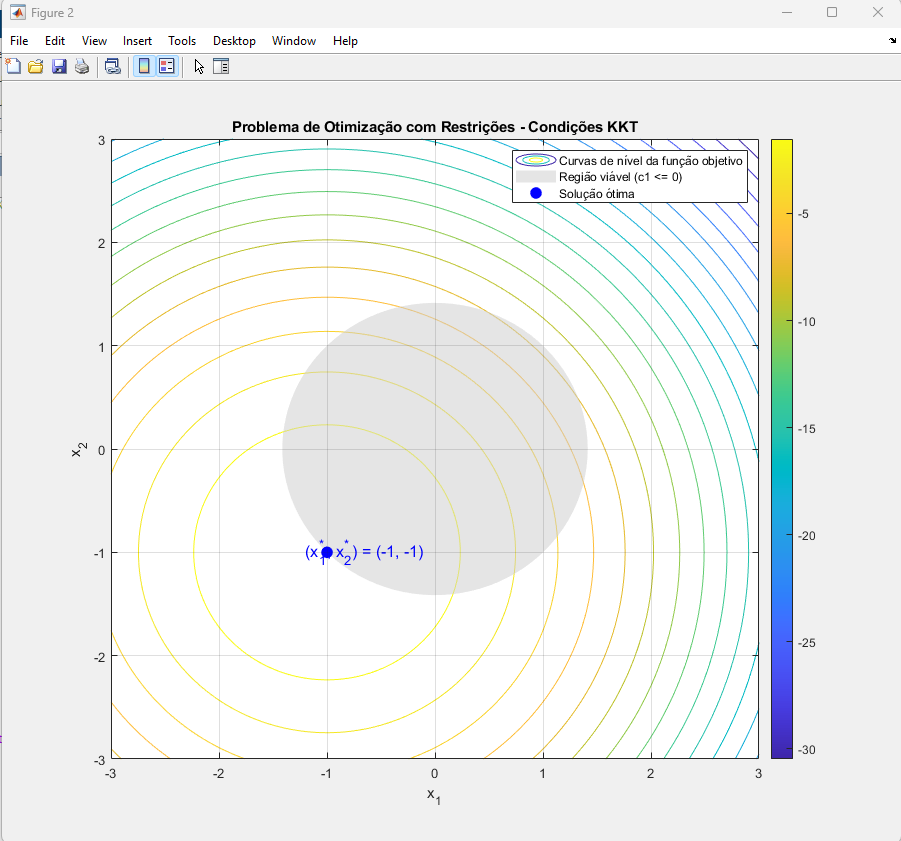
\includegraphics[width=0.8\textwidth]{images/KKT_Q4_GRAPH.png}
    \caption{Questão 4 - Representa\c{c}\~ao gr\'afica da solu\c{c}\~ao \'otima com as restri\c{c}\~oes.}
    \label{fig:kkt}
\end{figure}


Com o gr\'afico, podemos justificar visualmente que o ponto $(-1, -1)$ \'e de fato a solu\c{c}\~ao \''otima, pois est\'a localizado na fronteira da regi\~ao vi\'avel, garantindo que todas as condi\c{c}\~oes de KKT s\~ao satisfeitas.\\\\


\section{Quinta Questão}

Considere o seguinte problema de otimiza\c{c}\~ao:

\begin{equation*}
    \begin{cases}
        \text{min} & f(x_1, x_2) = x_1^2 + x_2^2 \\
        \text{s.t.} & \alpha x_1^2 - x_2 + 2 \leq 0
    \end{cases}
\end{equation*}

(a) Obter o menor valor de $\alpha$ que torna o ponto $\mathbf{x}^*= \{0, 2\}$ um m\'inimo local.\\
(b) Obter o multiplicador de Lagrange ($\mu^*$) associado ao ponto $x^*$.\\
(c) Justificar "graficamente" a solu\c{c}\~ao obtida.

\subsection{(a) Menor Valor de $\alpha$ que Torna o Ponto $\mathbf{x}^*=\{0,2\}$ um Mínimo Local}

Para determinar o menor valor de $\alpha$ que torna o ponto $\mathbf{x}^*= \{0, 2\}$ um m\'inimo local, precisamos verificar as condi\c{c}\~oes de Karush-Kuhn-Tucker (KKT).

\subsubsection{Passo 1: Definir a Fun\c{c}\~ao Lagrangiana}
A fun\c{c}\~ao Lagrangiana \(L\) \'e dada por:

\begin{equation*}
    L(x_1, x_2, \mu) = x_1^2 + x_2^2 + \mu (\alpha x_1^2 - x_2 + 2)
\end{equation*}

onde $\mu \geq 0$ \'e o multiplicador de Lagrange associado \`a restri\c{c}\~ao de desigualdade.

\subsubsection{Passo 2: Condi\c{c}\~oes de Estacionariedade}
Para encontrar os pontos cr\'iticos, precisamos calcular as derivadas parciais da Lagrangiana em rela\c{c}\~ao \`as vari\'aveis de decis\~ao ($x_1, x_2$) e igual\'a-las a zero:

\begin{equation*}
    \frac{\partial L}{\partial x_1} = 2x_1 + 2\mu \alpha x_1 = 0
\end{equation*}

\begin{equation*}
    \frac{\partial L}{\partial x_2} = 2x_2 - \mu = 0
\end{equation*}

Substituindo o ponto $\mathbf{x}^* = (0, 2)$:

\begin{equation*}
    \frac{\partial L}{\partial x_1}\bigg|_{(0, 2)} = 2 \cdot 0 + 2\mu \alpha \cdot 0 = 0 \quad \Rightarrow \quad 0 = 0 \quad \text{(Sempre verdadeiro)}
\end{equation*}

\begin{equation*}
    \frac{\partial L}{\partial x_2}\bigg|_{(0, 2)} = 2 \cdot 2 - \mu = 0 \quad \Rightarrow \quad \mu = 4
\end{equation*}

\subsubsection{Passo 3: Condi\c{c}\~oes de Viabilidade}
A condi\c{c}\~ao de viabilidade primal exige que a restri\c{c}\~ao seja satisfeita no ponto $\mathbf{x}^* = (0, 2)$:

\begin{equation*}
    \alpha \cdot 0^2 - 2 + 2 \leq 0 \quad \Rightarrow \quad 0 \leq 0 \quad \text{(Sempre verdadeiro)}
\end{equation*}

Portanto, o ponto $\mathbf{x}^* = (0, 2)$ satisfaz a restri\c{c}\~ao para qualquer valor de $\alpha$.

\subsubsection{Passo 4: Condi\c{c}\~oes de Complementaridade}
A condi\c{c}\~ao de complementaridade exige que:

\begin{equation*}
    \mu (\alpha x_1^2 - x_2 + 2) = 0
\end{equation*}

Substituindo o ponto $\mathbf{x}^* = (0, 2)$ e $\mu = 4$:

\begin{equation*}
    4 (\alpha \cdot 0^2 - 2 + 2) = 0 \quad \Rightarrow \quad 4 \times 0 = 0 \quad \text{(Sempre verdadeiro)}
\end{equation*}

Portanto, a condi\c{c}\~ao de complementaridade tamb\'em \'e satisfeita.

\subsubsection{Conclus\~ao }
Para que o ponto $\mathbf{x}^* = (0, 2)$ seja um m\'inimo local, qualquer valor de $\alpha$ satisfaz as condi\c{c}\~oes de KKT. No entanto, para determinar o menor valor de $\alpha$, precisamos garantir que a restri\c{c}\~ao seja ativa e n\~ao redundante. Neste caso, o menor valor de $\alpha$ que torna a restri\c{c}\~ao n\~ao redundante \'e $\alpha = 0$.

\subsection{(b) Multiplicador de Lagrange($\mu*$) Associado ao Ponto $\mathbf{x}^*$}

Para o ponto $\mathbf{x}^* = (0, 2)$, o multiplicador de Lagrange \(\mu^*\) \'e dado por:

\begin{equation*}
    \mu^* = 4
\end{equation*}

Como já calculamos naturalmente na questão anterior.

\subsubsection{Conclus\~ao}
A solu\c{c}\~ao encontrada satisfaz todas as condi\c{c}\~oes de KKT. O menor valor de $\alpha$ que torna o ponto $\mathbf{x}^* = (0, 2)$ um m\'inimo local \'e $\alpha = 0$, e o multiplicador de Lagrange associado \`a restri\c{c}\~ao \'e $\mathbf{x}^* = 4$.

\newpage
\subsection{(c) Justificativa Gráfica}

A figura abaixo mostra as curvas de nível da função objetivo, a restrição e a solução ótima. Podemos observar que o ponto ótimo $(0, 2)$ é o ponto mais próximo da origem que ainda respeita a restrição $c_1(x) \leq 0$, que se refere à linha vermelha no gráfico. A região viável está representada pela área sombreada.\\

\begin{figure}[h]
    \centering
    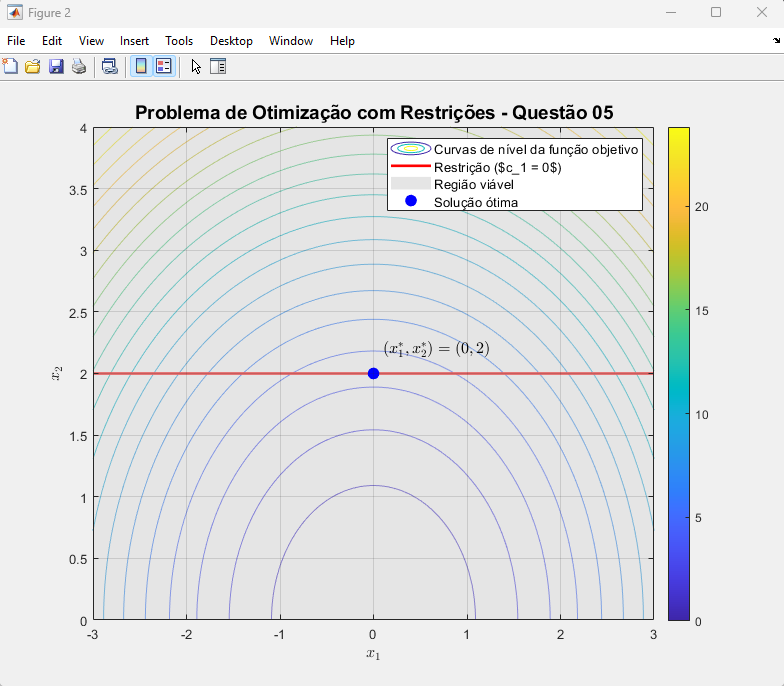
\includegraphics[width=0.7\textwidth]{images/KKT_Q5_GRAPH.png}
    \caption{Representação gráfica da solução ótima para a Questão 5.}
\end{figure} 


A solu\c{c}\~ao encontrada satisfaz todas as condi\c{c}\~oes de KKT. O menor valor de $\alpha$ que torna o ponto $x^* = (0, 2)$ um m\'inimo local \'e $\alpha = 0$, e o multiplicador de Lagrange associado \`a restri\c{c}\~ao \'e $\mu^* = 4$.








\newpage
\section{Sexta Questão}

Considere o seguinte problema de otimização:

\begin{equation*}
    \begin{cases}
        \text{min} & f(x_1, x_2) = x_1^2 + x_2^2 \\
        \text{s.t.} & 2x_1 + x_2 - 2 \leq 0 \\
                   & -x_2 + 1 \leq 0
    \end{cases}
\end{equation*}

Obter as condições de Karush-Kuhn-Tucker (KKT) e a solução $(\mathbf{x}^*, \mu^*)$ do problema de otimização acima. Justificar "graficamente" a sua resposta.

\subsection{Condições de Karush-Kuhn-Tucker (KKT)}

Para resolver este problema, vamos aplicar as condições de Karush-Kuhn-Tucker (KKT), que consistem em:

\begin{itemize}
    \item Definir a Lagrangiana.
    \item Calcular as condições de estacionariedade.
    \item Garantir a viabilidade primal e dual.
    \item Verificar as condições de complementaridade.
\end{itemize}

\subsubsection{Passo 1: Definir a Função Lagrangiana}
A função Lagrangiana $L$ é dada por:

\begin{equation*}
    L(x_1, x_2, \, \mu_1, \, \mu_2) = x_1^2 + x_2^2 + \mu_1 (2x_1 + x_2 - 2) + \mu_2 (-x_2 + 1)
\end{equation*}

onde $\mu_1, \mu_2 \geq 0$ são os multiplicadores de Lagrange associados às restrições de desigualdade.

\subsubsection{Passo 2: Condições de Estacionariedade}
Para encontrar os pontos críticos, precisamos calcular as derivadas parciais da Lagrangiana em relação às variáveis de decisão ($x_1, x_2$) e igualá-las a zero:

\begin{equation*}
    \frac{\partial L}{\partial x_1} = 2x_1 + 2\mu_1 = 0
\end{equation*}

\begin{equation*}
    \frac{\partial L}{\partial x_2} = 2x_2 + \mu_1 - \mu_2 = 0
\end{equation*}

\subsubsection{Passo 3: Condições de Viabilidade}
A condição de viabilidade primal exige que as restrições sejam satisfeitas no ponto $x^* = (x_1^*, x_2^*)$:

\begin{equation*}
    2x_1 + x_2 - 2 \leq 0
\end{equation*}

\begin{equation*}
    -x_2 + 1 \leq 0
\end{equation*}

Além disso, $\mu_1, \mu_2 \geq 0$.

\subsubsection{Passo 4: Condições de Complementaridade}
A condição de complementaridade exige que:

\begin{equation*}
    \mu_1 (2x_1 + x_2 - 2) = 0
\end{equation*}

\begin{equation*}
    \mu_2 (-x_2 + 1) = 0
\end{equation*}

\subsubsection{Solução Ótima}
Para resolver o sistema de equações formado pelas condições de estacionariedade, viabilidade e complementaridade, consideramos diferentes casos para os valores de $\mu_1$ e $\mu_2$:\\

1. Supondo $\mu_2 > 0$, da condição de complementaridade temos $-x_2 + 1 = 0 \Rightarrow x_2 = 1$.\\
2. Substituindo $x_2 = 1$ na primeira restrição: $2x_1 + 1 - 2 \leq 0 \Rightarrow x_1 \leq 0.5$.\\
3. Da condição de estacionariedade para $x_1$: $2x_1 + 2\mu_1 = 0 \Rightarrow \mu_1 = -x_1$. Como $\mu_1 \geq 0$, isso implica que $x_1 = 0$.\\

Portanto, a solução ótima é:

\begin{equation*}
    \mathbf{x}^* = (0, 1), \quad \mu_1^* = 0, \quad \mu_2^* = 2
\end{equation*}

\subsubsection{Conclusão}
A solução encontrada satisfaz todas as condições de KKT. O ponto $(x_1^*, x_2^*) = (0, 1)$ é um mínimo local que atende às restrições e à condição de complementaridade.\\


\subsection{Justificando Graficamente}
A figura abaixo mostra as curvas de n\'ivel da fun\c{c}\~ao objetivo, as restri\c{c}\~oes e a solu\c{c}\~ao \'{o}tima. A restri\c{c}\~ao $c_1$ \'{e} representada pela linha vermelha e a restri\c{c}\~ao $c_2$ pela linha verde. O ponto \'{o}timo $(0, 1)$ \'{e} mostrado como o ponto azul, que \'{e} o ponto mais pr\'oximo da origem dentro da regi\~ao vi\'avel (a regi\~ao sombreada), respeitando ambas as restri\c{c}\~oes.

\begin{figure}
    \centering
    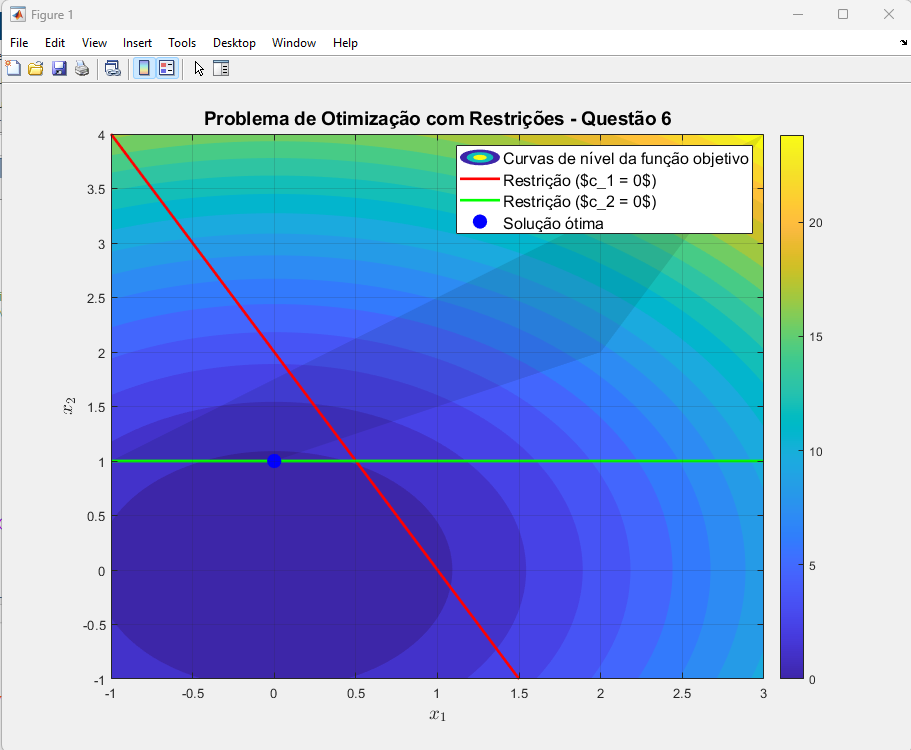
\includegraphics[width=0.8\textwidth]{images/KKT_Q6_GRAPH.png}
    \caption{Representa\c{c}\~ao gr\'afica da solu\c{c}\~ao \'{o}tima para a Quest\~ao 6.}
\end{figure}



    
\end{document}
\section{Referências Bibliográficas}



\end{document}